%----------------------------------------------------------------------------------------
% HET PROJECTIEVE VLAK: perspectief, punten op oneindig, homogene coördinaten, snijpunt en
% verbindingsrechte, Desargues, projectieve transformaties, Pappus. Alle opgaven zijn eigen werk.
%
% Opbouw: Probleem, Start, leerstof, en op een nieuwe pagina de Opdrachten, Koppel en Test jezelf.
% Labels van dit hoofdstuk beginnen met h2-.
%----------------------------------------------------------------------------------------

\mychapter{2}{Het projectieve vlak}

\begin{probleem}
\naast{Een schilder zet een vloer met vierkante tegels op zijn doek. De voegen die van hem weg lopen, zijn op de vloer evenwijdig, maar op het doek lopen ze samen in één punt $V$. Ook de diagonalen van de tegels lopen samen, in een ander punt $D$. Waar liggen $V$ en $D$ op het doek? Waarom liggen ze op één horizontale rechte, de horizon? En bestaat er een meetkunde waarin evenwijdige rechten elkaar echt snijden?}{\begin{tikzpicture}[scale=1.6,font=\scriptsize]
  \begin{scope}
    \clip (-1.25,-1.05) rectangle (1.25,0);
    \foreach \k in {-6,...,6}{\draw[grijs] ({\k},-1) -- (0,0);}
    \foreach \z in {1,2,3,4,5,6,8,10,14,20}{\draw[grijs] (-1.3,{-1/\z}) -- (1.3,{-1/\z});}
    \foreach \c in {-4,...,1}{\draw[accent,thick] ({1+\c},-1) -- (1,0);}
  \end{scope}
  \draw[thick] (-1.25,0) -- (1.25,0) node[right] {horizon};
  \fill (0,0) circle (1.2pt) node[above] {$V$};
  \fill[accent] (1,0) circle (1.4pt) node[above,text=black] {$D$};
\end{tikzpicture}}
\end{probleem}

\lkr{Leerplan Complementair: LPD 15 (projectieve coördinaten), met de wenken over punten op oneindig, homogene coördinaten, snijpunten van rechten en de stellingen van Pappus en Desargues. Voorkennis uit pakket 4: Matrices (determinant van een $3 \times 3$-matrix, homogene stelsels), Ruimtemeetkunde (rechten en vlakken door de oorsprong), en hoofdstuk 1. Het vectorproduct is geen voorkennis: het wordt hier ingevoerd als rekenregel met een determinant.}

In het vlak snijden twee rechten elkaar in één punt, behalve als ze evenwijdig zijn. Die uitzondering kost overal een geval extra: in hoofdstuk 1 gingen drie rechten \textit{door één punt of waren ze evenwijdig}. Schilders uit de renaissance losten het anders op: op hun doek snijden evenwijdige rechten elkaar wel, op de horizon. In dit hoofdstuk maken we daar wiskunde van. We voegen aan het vlak punten op oneindig toe, en beschrijven alle punten met drie coördinaten. Dan snijden twee rechten elkaar altijd, en worden bewijzen over rechten en punten kort en mooi.

\begin{oefeningen}[Start]
\oef{h2-start-1}

\oef{h2-verken}
\end{oefeningen}

%========================================================================================
\section{Punten op oneindig}

\subsection{Perspectief}

Hoe tekent een schilder wat hij ziet? Hij kijkt met één oog door een glazen plaat, het doek, en zet elk punt van de ruimte op de plaats waar de lichtstraal naar zijn oog het doek doorprikt. Leg het oog $O$ in de oorsprong, kijk in de richting van de $z$-as, en zet het doek in het vlak $z = 1$, met de $y$-as naar boven. De lichtstraal naar het punt $P(X, Y, Z)$, met $Z > 0$, is de rechte $OP$: de punten $t\,(X, Y, Z)$. Ze prikt het doek door bij $t = \tfrac1Z$, dus in het punt
\[ \Bigl(\frac XZ, \frac YZ\Bigr) . \]
Alle punten op dezelfde lichtstraal geven hetzelfde punt op het doek: het oog ziet ze achter elkaar.

\figuren{\begin{tikzpicture}[xscale=1.15,yscale=1.7,font=\scriptsize]
  \draw[thick] (-.2,-1) -- (6.3,-1) node[right] {vloer, $y = -1$};
  \draw[accent!60,line width=2pt] (1,-1.2) -- (1,.55) node[above,text=black] {doek, $z = 1$};
  \draw[grijs,dashed] (0,0) -- (6.3,0) node[right,text=black] {ooghoogte};
  \foreach \z in {1.5,3,6}{\draw[grijs] (0,0) -- (\z,-1); \fill (\z,-1) circle (1.3pt); \fill[accent] (1,{-1/\z}) circle (1.3pt);}
  \fill (0,0) circle (1.5pt) node[left] {$O$};
  \fill[accent] (1,0) circle (1.5pt) node[above right,text=black] {$H$};
  \node[below] at (1.5,-1) {$Z = 1{,}5$};
  \node[below] at (3,-1) {$Z = 3$};
  \node[below] at (6,-1) {$Z = 6$};
\end{tikzpicture}}
\begin{center}\small Zijaanzicht: hoe verder een punt van de vloer, hoe dichter zijn beeld bij de ooghoogte $H$.\end{center}

Een punt van de vloer op afstand $Z$ komt op hoogte $-\tfrac1Z$ op het doek. Hoe verder het punt, hoe dichter bij hoogte 0, maar het bereikt die nooit: de lichtstraal op ooghoogte loopt evenwijdig met de vloer. Wat gebeurt er met een hele rechte?

\begin{theorie}
\begin{stelling}{Verdwijnpunt}
Bekijk de rechten in de ruimte met richtingsvector $(a, b, c)$, met $c > 0$. Hoe verder je langs zo'n rechte gaat, hoe dichter haar beeld op het doek komt bij het punt

\vspace{1mm}
\qquad $\formule{\Bigl(\dfrac ac, \dfrac bc\Bigr)}$

\vspace{1mm}
Dat punt hangt alleen af van de richting: evenwijdige rechten hebben hetzelfde \textbf{\textcolor{accent}{verdwijnpunt}}.
\end{stelling}

\begin{bewijs}
De rechte door $(X_0, Y_0, Z_0)$ bestaat uit de punten $(X_0 + ta, Y_0 + tb, Z_0 + tc)$, met beeld
\bewijsregel{\Bigl(\frac{X_0 + ta}{Z_0 + tc}, \frac{Y_0 + tb}{Z_0 + tc}\Bigr) = \Bigl(\frac{X_0/t + a}{Z_0/t + c}, \frac{Y_0/t + b}{Z_0/t + c}\Bigr) \ \to \ \Bigl(\frac ac, \frac bc\Bigr) \quad \text{als } t \to +\infty .}
\end{bewijs}
\end{theorie}

Voor rechten in de vloer is $b = 0$: hun verdwijnpunt $\bigl(\tfrac ac, 0\bigr)$ ligt op de rechte $y = 0$ van het doek, de horizon.

\voorbeeld{}{Op de vloer liggen twee rechte straten die elkaar loodrecht kruisen: de ene met richting $(1, 0, 2)$, de andere met richting $(-2, 0, 1)$. Langs de straten staan verticale lantaarnpalen, met richting $(0, 1, 0)$. Het oog staat op hoogte 1 boven de vloer en het doek staat op afstand 1. Waar liggen de verdwijnpunten van de straten en van de palen?\label{vb:h2-verdwijn}}{%
\uitleg{Lees het verdwijnpunt telkens af met de stelling.}
\begin{stappen}
(1, 0, 2) \ \to \ \bigl(\tfrac12, 0\bigr) & De eerste straat: op de horizon. \\[1ex]
(-2, 0, 1) \ \to \ (-2, 0) & De tweede straat: ook op de horizon. \\[1ex]
(0, 1, 0): \ c = 0 & De palen: geen verdwijnpunt.
\end{stappen}
De palen staan evenwijdig met het doek. Een paal in het punt $(X_0, -1, Z_0)$ komt op het doek op de rechte $x = \tfrac{X_0}{Z_0}$: de beelden van de palen blijven verticaal en evenwijdig.}

\begin{oefeningen}
\oef{h2-persp}
\end{oefeningen}

\subsection{Het projectieve vlak}

Op het doek snijden de beelden van evenwijdige rechten elkaar in hun verdwijnpunt. Dat punt is het beeld van geen enkel punt van de vloer: het is alsof de rechten elkaar \textit{oneindig ver} snijden. Dat idee maken we exact. Het vlak krijgt voor elke richting één extra punt, dat op alle rechten van die richting ligt.

\begin{theorie}
Voeg aan het vlak voor elke richting een \textbf{\textcolor{accent}{punt op oneindig}} toe, dat op alle rechten met die richting ligt. Alle punten op oneindig samen vormen een nieuwe rechte, de \textbf{\textcolor{accent}{rechte op oneindig}}. Het vlak met die punten en die rechte erbij heet het \textbf{\textcolor{accent}{projectieve vlak}}.
\end{theorie}

Een gewone rechte krijgt zo één punt op oneindig erbij, en evenwijdige rechten hebben hetzelfde punt op oneindig. In een tekening kun je dat punt niet zien, maar op het doek van de schilder wel: daar is het het verdwijnpunt. Het grote voordeel staat in de volgende stelling: er zijn geen uitzonderingen meer.

\begin{theorie}
\begin{stelling}{Snijpunt en verbindingsrechte}
In het projectieve vlak hebben twee verschillende rechten precies één gemeenschappelijk punt, en liggen twee verschillende punten op precies één rechte.
\end{stelling}

\begin{bewijs}
\textit{Twee rechten.} Twee gewone rechten die niet evenwijdig zijn, snijden elkaar in één gewoon punt, en hebben verschillende punten op oneindig. Twee evenwijdige rechten hebben geen gewoon punt gemeen, en wel hetzelfde punt op oneindig. Een gewone rechte en de rechte op oneindig hebben alleen het punt op oneindig van de gewone rechte gemeen.

\textit{Twee punten.} Twee gewone punten liggen op één gewone rechte, en op de rechte op oneindig niet. Een gewoon punt $P$ en het punt op oneindig van een richting $\vec v$ liggen alleen op de rechte door $P$ met richting $\vec v$. Twee punten op oneindig liggen alleen op de rechte op oneindig, want een gewone rechte heeft maar één punt op oneindig.
\end{bewijs}
\end{theorie}

De twee helften van de stelling lijken op elkaar: wissel \textit{punt} en \textit{rechte}, en \textit{ligt op} en \textit{gaat door}, en de ene wordt de andere. Dat heet \emph{dualiteit}. In de volgende sectie zie je dat het meer is dan een toevalligheid.

\begin{oefeningen}
\oef{h2-oneindig}
\end{oefeningen}

%========================================================================================
\section{Homogene coördinaten}

\subsection{Punten}

Hoe geef je een punt op oneindig coördinaten? Kijk opnieuw naar het oog van de schilder. Elk punt van het doek hoort bij één lichtstraal door $O$, en die kun je beschrijven met elk punt $(x, y, z) \neq (0, 0, 0)$ erop. Het doekpunt $(2, 3)$ hoort bij de rechte door $O$ en $(2, 3, 1)$, maar ook $(4, 6, 2)$ of $(-2, -3, -1)$ ligt op die rechte. En de rechten door $O$ die evenwijdig zijn met het doek, met $z = 0$, prikken het doek niet door: dat zijn de richtingen zonder doekpunt, de punten op oneindig.

\begin{theorie}
Een punt van het projectieve vlak heeft \textbf{\textcolor{accent}{homogene coördinaten}} $\formule{\hc xyz}$, met $(x, y, z) \neq (0, 0, 0)$. Daarbij is $\hc xyz = \hc{kx}{ky}{kz}$ voor elk getal $k \neq 0$.
\begin{itemize}
\item Het gewone punt $(x, y)$ heeft homogene coördinaten $\formule{\hc xy1}$. Omgekeerd is $\hc xyz$ met $z \neq 0$ het punt $\Bigl(\dfrac xz, \dfrac yz\Bigr)$.
\item Het punt op oneindig met richting $(x, y)$ heeft homogene coördinaten $\formule{\hc xy0}$.
\end{itemize}
\end{theorie}

De dubbelpunten herinneren eraan dat alleen de verhoudingen tellen: $\hc246$ en $\hc123$ zijn hetzelfde punt. Dat past bij de richtingen: $(1, 2)$ en $(-3, -6)$ zijn dezelfde richting, en $\hc120 = \hc{-3}{-6}0$.

\voorbeeld{}{Geef homogene coördinaten van $(3, -2)$ en van het punt op oneindig van de rechte $y = 4x$. Welk punt is $\hc{4}{6}{2}$? En $\hc{2}{-1}{0}$?\label{vb:h2-hc}}{%
\uitleg{Een gewoon punt krijgt een 1 achteraan; een punt op oneindig een 0, met de richting vooraan.}
\begin{stappen}
(3, -2) \ \to \ \hc{3}{-2}{1} = \hc{6}{-4}{2} & Elk veelvoud mag. \\[1ex]
\text{richting } (1, 4) \ \to \ \hc140 & Het punt op oneindig van $y = 4x$. \\[1ex]
\hc462 \ \to \ \bigl(\tfrac42, \tfrac62\bigr) = (2, 3) & Deel door de derde coördinaat. \\[1ex]
\hc{2}{-1}{0} & Het punt op oneindig met richting $(2, -1)$.
\end{stappen}}

\begin{werkwijze}
Van gewoon naar homogeen: $(x, y) \to \hc xy1$. Van homogeen naar gewoon: is de derde coördinaat niet 0, deel er dan door; is ze 0, dan is het een punt op oneindig, met de richting in de eerste twee coördinaten.
\end{werkwijze}

\nujij{Zijn $\hc{1}{-2}{3}$ en $\hc{-3}{6}{-9}$ hetzelfde punt? Welk?}{Ja, maal $-3$: het punt $\bigl(\tfrac13, -\tfrac23\bigr)$.}

\begin{oefeningen}
\oef{h2-hc}
\end{oefeningen}

\subsection{Rechten}

Wat wordt de vergelijking van een rechte? Vul in $ax + by + c = 0$ de coördinaten $\tfrac xz$ en $\tfrac yz$ in, en vermenigvuldig met $z$. Dan staat er $ax + by + cz = 0$: elke term heeft graad 1, de vergelijking is \emph{homogeen}. Ze geldt voor $\hc xyz$ als en slechts als ze geldt voor $\hc{kx}{ky}{kz}$, en dat moet ook: het is hetzelfde punt.

\begin{theorie}
\begin{stelling}{Vergelijking van een rechte}
Elke rechte van het projectieve vlak heeft een vergelijking

\vspace{1mm}
\qquad $\formule{ax + by + cz = 0}$ \qquad met $(a, b, c) \neq (0, 0, 0)$,

\vspace{1mm}
en elke zulke vergelijking stelt een rechte voor. De gewone rechte $ax + by + c = 0$ krijgt zo de vergelijking $ax + by + cz = 0$, en de rechte op oneindig is $\formule{z = 0}$.
\end{stelling}

\begin{bewijs}
De gewone punten $\hc xy1$ van $ax + by + cz = 0$ zijn de punten van $ax + by + c = 0$. Haar punten op oneindig zijn de $\hc xy0$ met $ax + by = 0$: dat is alleen $\hc{-b}{a}{0}$, het punt op oneindig met de richting $(-b, a)$ van de rechte. De vergelijking geeft dus precies de gewone rechte met haar punt op oneindig. De vergelijking $z = 0$, of $0x + 0y + 1z = 0$, bevat alle punten op oneindig en geen enkel gewoon punt. Omgekeerd: is $(a, b) \neq (0, 0)$, dan is $ax + by + cz = 0$ een gewone rechte, anders is ze $cz = 0$ met $c \neq 0$, de rechte op oneindig.
\end{bewijs}
\end{theorie}

Ook de vergelijking ligt maar vast op een factor na: $2x - y + 3z = 0$ en $4x - 2y + 6z = 0$ zijn dezelfde rechte. Daarom noteren we de rechte als $\rc{2}{-1}{3}$, met vierkante haken om ze van een punt te onderscheiden. Dat punt $\hc xyz$ op de rechte $\rc abc$ ligt, betekent dan $ax + by + cz = 0$: een scalair product dat 0 is.

\voorbeeld{}{Geef de homogene vergelijking van de rechte $y = 2x + 3$ en haar punt op oneindig. Welke gewone rechte is $x - 4z = 0$?\label{vb:h2-rechte}}{%
\uitleg{Breng alles naar één lid, en geef de constante een $z$.}
\begin{stappen}
2x - y + 3 = 0 \ \to \ 2x - y + 3z = 0 & De rechte $\rc{2}{-1}{3}$. \\[1ex]
2x - y = 0 \text{ met } z = 0 \ \to \ \hc120 & Haar punt op oneindig: de richting $(1, 2)$. \\[1ex]
x - 4z = 0 \ \to \ x = 4 & Een verticale rechte, met punt op oneindig $\hc010$.
\end{stappen}}

\begin{oefeningen}
\oef{h2-rechte}
\end{oefeningen}

\subsection{Snijpunt en verbindingsrechte}

Het snijpunt van twee rechten $\rc abc$ en $\rc{a'}{b'}{c'}$ vind je met het stelsel $ax + by + cz = 0$ en $a'x + b'y + c'z = 0$. Dat zijn twee vergelijkingen met drie onbekenden: de oplossingen vormen een rechte door de oorsprong van de ruimte, en dat is precies één punt van het projectieve vlak. Er is een formule voor, en ze heeft een naam.

\begin{theorie}
Het \textbf{\textcolor{accent}{vectorproduct}} van $u = (u_1, u_2, u_3)$ en $v = (v_1, v_2, v_3)$ is

\vspace{1mm}
\qquad $\formule{u \times v = (u_2v_3 - u_3v_2,\ u_3v_1 - u_1v_3,\ u_1v_2 - u_2v_1)}$
\end{theorie}

Je onthoudt het met een determinant. Voor elke $w$ is, ontwikkeld naar de eerste rij,
\[ w \cdot (u \times v) = \begin{vmatrix} w_1 & w_2 & w_3 \\ u_1 & u_2 & u_3 \\ v_1 & v_2 & v_3 \end{vmatrix} . \]
De drie componenten van $u \times v$ zijn dus de $2 \times 2$-determinanten die je krijgt door telkens één kolom van de onderste twee rijen te schrappen, met een minteken in het midden.

\begin{theorie}
\begin{stelling}{Snijpunt en verbindingsrechte berekenen}
De rechten $l$ en $m$ snijden elkaar in het punt $\formule{l \times m}$. De punten $P$ en $Q$ liggen op de rechte $\formule{P \times Q}$.
\end{stelling}

\begin{bewijs}
Met de determinant is $l \cdot (l \times m) = \begin{vmatrix} l \\ l \\ m \end{vmatrix} = 0$ en $m \cdot (l \times m) = \begin{vmatrix} m \\ l \\ m \end{vmatrix} = 0$, want een determinant met twee gelijke rijen is 0. Het punt $l \times m$ ligt dus op beide rechten. Het is geen nulvector: $l$ en $m$ zijn geen veelvouden van elkaar, dus de matrix met rijen $l$ en $m$ heeft rang 2, en een van haar $2 \times 2$-determinanten, de componenten van $l \times m$, is niet 0. Voor twee punten is de berekening dezelfde, met $P$ en $Q$ in de plaats van $l$ en $m$.
\end{bewijs}
\end{theorie}

\voorbeeld{}{Bepaal het snijpunt van de evenwijdige rechten $x + 2y = 3$ en $x + 2y = 7$.\label{vb:h2-snij}}{%
\uitleg{In het gewone vlak is er geen snijpunt. In homogene coördinaten wel: neem het vectorproduct.}
\begin{stappenbreed}
\rc{1}{2}{-3} \times \rc{1}{2}{-7} & De rechten $x + 2y - 3z = 0$ en $x + 2y - 7z = 0$. \\[1ex]
= \bigl(2 \cdot (-7) - (-3) \cdot 2,\ (-3) \cdot 1 - 1 \cdot (-7),\ 1 \cdot 2 - 2 \cdot 1\bigr) & De formule. \\[1ex]
= (-8, 4, 0) \ \to \ \hc{-2}{1}{0} & Een punt op oneindig.
\end{stappenbreed}
De richting $(-2, 1)$ is de richting van beide rechten, zoals het moet.}

\voorbeeld{}{Bepaal een vergelijking van de rechte door $(1, 2)$ en het punt op oneindig $\hc310$.\label{vb:h2-verbind}}{%
\uitleg{Dezelfde formule, nu met twee punten.}
\begin{stappenbreed}
\hc121 \times \hc310 = (2 \cdot 0 - 1 \cdot 1,\ 1 \cdot 3 - 1 \cdot 0,\ 1 \cdot 1 - 2 \cdot 3) & De formule. \\[1ex]
= (-1, 3, -5) & De rechte $-x + 3y - 5z = 0$. \\[1ex]
x - 3y + 5 = 0 & In gewone coördinaten.
\end{stappenbreed}
Controle: $(1, 2)$ ligt erop, want $1 - 6 + 5 = 0$, en de richting is $(3, 1)$. Het is de rechte door $(1, 2)$ met richtingsvector $(3, 1)$.}

\begin{werkwijze}
Schrijf de rechten of de punten in homogene coördinaten en neem hun vectorproduct. Voor twee rechten krijg je het snijpunt, voor twee punten de coëfficiënten van de verbindingsrechte. Zet het resultaat om naar gewone coördinaten als dat kan.
\end{werkwijze}

\nujij{Bepaal het snijpunt van $y = 3$ met de rechte op oneindig.}{$\rc{0}{1}{-3} \times \rc001 = (1, 0, 0)$: het punt op oneindig van de $x$-richting.}

\begin{oefeningen}
\oef{h2-snij}
\end{oefeningen}

\subsection{Op één rechte en door één punt}

In hoofdstuk 1 testte je met een determinant of drie punten op één rechte liggen. De rijen waren $(x_i, y_i, 1)$: dat waren al homogene coördinaten. En bij drie rechten moest je \textit{of evenwijdig} toevoegen. In het projectieve vlak worden de twee tests één en dezelfde.

\begin{theorie}
\begin{stelling}{Op één rechte}
Drie punten $P$, $Q$ en $R$ liggen op één rechte als en slechts als \qquad $\formule{\begin{vmatrix} P \\ Q \\ R \end{vmatrix} = 0}$
\end{stelling}

\begin{bewijs}
De punten liggen op de rechte $l \neq (0, 0, 0)$ als en slechts als $P \cdot l = Q \cdot l = R \cdot l = 0$, dus als het homogene stelsel met de rijen $P$, $Q$ en $R$ een oplossing $l$ heeft die niet nul is. Dat is zo als en slechts als de determinant 0 is.
\end{bewijs}
\end{theorie}

\begin{theorie}
\begin{stelling}{Door één punt}
Drie rechten $l$, $m$ en $n$ gaan door één punt als en slechts als \qquad $\formule{\begin{vmatrix} l \\ m \\ n \end{vmatrix} = 0}$
\end{stelling}

\begin{bewijs}
Hetzelfde bewijs, met de rollen van punten en rechten omgewisseld: de rechten gaan door het punt $X \neq (0, 0, 0)$ als en slechts als $l \cdot X = m \cdot X = n \cdot X = 0$.
\end{bewijs}
\end{theorie}

Het \textit{of evenwijdig} uit hoofdstuk 1 is verdwenen: drie evenwijdige rechten gaan nu door één punt, hun gemeenschappelijke punt op oneindig. De twee stellingen zijn elkaars duale. In het projectieve vlak is dat een algemene regel, het \emph{dualiteitsprincipe}: elke stelling over punten en rechten blijft waar als je \textit{punt} en \textit{rechte} wisselt, want de formules voor punten en rechten zijn dezelfde.

\voorbeeld{}{Liggen $\hc121$, $\hc310$ en $\hc431$ op één rechte? Welke rechte?\label{vb:h2-det}}{%
\uitleg{Bereken de determinant, en daarna de rechte met het vectorproduct van twee van de punten.}
\begin{stappen}
\begin{vmatrix} 1 & 2 & 1 \\ 3 & 1 & 0 \\ 4 & 3 & 1 \end{vmatrix} = 1 \cdot 1 - 2 \cdot 3 + 1 \cdot 5 = 0 & Ontwikkel naar de eerste rij: ja. \\[4ex]
\hc121 \times \hc310 = (-1, 3, -5) & Uit voorbeeld~\ref{vb:h2-verbind}.
\end{stappen}
Het is de rechte $x - 3y + 5 = 0$: $(4, 3)$ ligt erop, want $4 - 9 + 5 = 0$. Dat kon je ook zien: $(4, 3, 1) = (1, 2, 1) + (3, 1, 0)$.}

\nujij{Gaan de rechten $x = 1$, $x = 5$ en $z = 0$ door één punt?}{$\begin{vmatrix} 1 & 0 & -1 \\ 1 & 0 & -5 \\ 0 & 0 & 1 \end{vmatrix} = 0$: ja, door $\hc010$.}

\begin{oefeningen}
\oef{h2-det}
\end{oefeningen}

%========================================================================================
\section{Desargues en Pappus}

\subsection{De stelling van Desargues}

Girard Desargues (1591-1661) was ingenieur en architect in Lyon. Hij schreef over perspectief voor schilders en steenhouwers, en voerde daarbij als eerste punten op oneindig in. Zijn bekendste stelling gaat over twee driehoeken die \textit{in perspectief} staan: de rechten door overeenkomstige hoekpunten gaan door één punt $O$, zoals lichtstralen door een oog. Wat valt er dan op aan de overeenkomstige zijden?

\begin{theorie}
\begin{stelling}{Desargues}
Neem twee driehoeken $ABC$ en $A'B'C'$ zodat $AA'$, $BB'$ en $CC'$ door één punt $O$ gaan. Dan liggen de snijpunten

\vspace{1mm}
\qquad $P = BC \cap B'C'$, \quad $Q = CA \cap C'A'$, \quad $R = AB \cap A'B'$

\vspace{1mm}
op één rechte.
\end{stelling}

\begin{bewijs}
Noem $o$, $a$, $a'$, \dots\ homogene coördinaten van de punten (met $O$ verschillend van de hoekpunten). Omdat $O$, $A$ en $A'$ op één rechte liggen, is $o$ een combinatie van $a$ en $a'$. Kies de veelvouden van $a$ en $a'$ zo dat $o = a - a'$, en net zo voor de andere twee:
\bewijsregel{o = a - a' = b - b' = c - c' .}
Dan is $a - b = a' - b'$. Het linkerlid ligt op $AB$, want $\det(a, b, a - b) = 0$, en het rechterlid op $A'B'$. Het is niet de nulvector, want $A \neq B$. Dus is $r = a - b$ het snijpunt $R$. Net zo is $p = b - c$ het punt $P$ en $q = c - a$ het punt $Q$. Maar
\bewijsregel{p + q + r = (b - c) + (c - a) + (a - b) = 0 ,}
zodat de rijen $p$, $q$, $r$ afhankelijk zijn: hun determinant is 0, en $P$, $Q$ en $R$ liggen op één rechte.
\end{bewijs}
\end{theorie}

\figuren{\begin{tikzpicture}[scale=.82,font=\scriptsize]
  \draw[grijs] (0,1.2) -- (3.68,-1.1) (0,1.2) -- (2.52,2.32) (0,1.2) -- (4.68,.84);
  \draw[accent,thick] (-.4,3.79) -- (6.7,3.95);
  \draw[lijngrijs,dashed] (1.8,2) -- (.36,3.8) (2.52,2.32) -- (.36,3.8);
  \draw[lijngrijs,dashed] (2.6,1) -- (6.28,3.944) (4.68,.84) -- (6.28,3.944);
  \draw[lijngrijs,dashed] (1.8,2) -- (2.004,3.84) (2.52,2.32) -- (2.004,3.84);
  \draw[thick] (1.6,.2) -- (1.8,2) -- (2.6,1) -- cycle;
  \draw[thick] (3.68,-1.1) -- (2.52,2.32) -- (4.68,.84) -- cycle;
  \punt[left]{0}{1.2}{O}
  \punt[below]{1.6}{.2}{A}
  \punt[above left]{1.8}{2}{B}
  \punt[below]{2.6}{1}{C}
  \punt[below]{3.68}{-1.1}{A'}
  \punt[right]{2.52}{2.32}{B'}
  \punt[right]{4.68}{.84}{C'}
  \fpunt[above]{.36}{3.8}{P}
  \fpunt[above]{6.28}{3.944}{Q}
  \fpunt[above]{2.004}{3.84}{R}
\end{tikzpicture}}
\begin{center}\small Twee driehoeken in perspectief vanuit $O$: de snijpunten van overeenkomstige zijden liggen op één rechte.\end{center}

Het bewijs gebruikt geen enkel geval apart: ook als twee overeenkomstige zijden evenwijdig zijn, werkt het, met een snijpunt op oneindig. In de ruimte is de stelling bijna vanzelfsprekend. Liggen de twee driehoeken in verschillende vlakken, dan snijden de verlengden van overeenkomstige zijden elkaar op de snijlijn van die twee vlakken (opdracht~\ref{oef:h2-o18}). De vlakke stelling is zo het perspectiefbeeld van de ruimtelijke.

\voorbeeld{}{Neem $O(0, 0)$, $A(2, 0)$, $B(0, 2)$, $C(1, 3)$, en $A'(4, 0)$, $B'(0, 3)$, $C'(2, 6)$ op de rechten $OA$, $OB$ en $OC$. Bereken $P$, $Q$ en $R$, en ga na dat ze op één rechte liggen.\label{vb:h2-desargues}}{%
\uitleg{Bereken elke zijde als vectorproduct van twee hoekpunten, en elk snijpunt als vectorproduct van twee zijden.}
\begin{stappenbreed}
AB = \hc201 \times \hc021 = \rc{-2}{-2}{4} \sim \rc{1}{1}{-2} & $x + y = 2$. \\[1ex]
A'B' = \hc401 \times \hc031 = \rc{-3}{-4}{12} & $3x + 4y = 12$. \\[1ex]
R = \rc{1}{1}{-2} \times \rc{-3}{-4}{12} = (4, -6, -1) \sim \hc{-4}{6}{1} & $R(-4, 6)$. \\[1ex]
BC = \rc{-1}{1}{-2}, \quad B'C' = \rc{-3}{2}{-6} & Net zo. \\[1ex]
P = \rc{-1}{1}{-2} \times \rc{-3}{2}{-6} = \hc{-2}{0}{1} & $P(-2, 0)$. \\[1ex]
CA = \rc{3}{1}{-6}, \quad C'A' = \rc{6}{2}{-24} & $3x + y = 6$ en $3x + y = 12$. \\[1ex]
Q = \rc{3}{1}{-6} \times \rc{6}{2}{-24} = (-12, 36, 0) \sim \hc{-1}{3}{0} & $CA \parallel C'A'$: $Q$ ligt op oneindig. \\[1ex]
\begin{vmatrix} -4 & 6 & 1 \\ -2 & 0 & 1 \\ -1 & 3 & 0 \end{vmatrix} = 12 - 6 - 6 = 0 & Op één rechte.
\end{stappenbreed}
De rechte $PR$ heeft richting $(-2, 6)$, dezelfde als $CA$: ze gaat door het punt op oneindig $Q$. Zonder punten op oneindig zou de stelling hier niets zeggen.}

\figuren{\begin{tikzpicture}[scale=.5,font=\scriptsize]
  \rooster{-5}{1}{4}{-1}{1}{6}
  \draw[accent,thick] (-4.5,7.5) -- (-1.75,-.75);
  \draw[grijs] (2,0) -- (-4,6) (4,0) -- (-4,6) (1,3) -- (-2,0) (2,6) -- (-2,0);
  \draw[accent!70,dashed,thick] (2.3,-.9) -- (.7,3.9) (4.3,-.9) -- (1.7,6.9);
  \draw[thick] (2,0) -- (0,2) -- (1,3) -- cycle;
  \draw[thick] (4,0) -- (0,3) -- (2,6) -- cycle;
  \punt[below right]{2}{0}{A}
  \punt[below left]{0}{2}{B}
  \punt[right]{1}{3}{C}
  \punt[below]{4}{0}{A'}
  \punt[left]{0}{3}{B'}
  \punt[right]{2}{6}{C'}
  \fpunt[below]{-2}{0}{P}
  \fpunt[left]{-4}{6}{R}
\end{tikzpicture}}
\begin{center}\small Het voorbeeld: $CA$ en $C'A'$ (gestippeld) zijn evenwijdig, en de rechte $PR$ ook.\end{center}

\begin{oefeningen}
\oef{h2-desargues}
\end{oefeningen}

\subsection{Projectieve transformaties}

In hoofdstuk 1 koos je met een affiene transformatie de handigste driehoek. Kan dat ook in het projectieve vlak, en hoe ver gaat dat? Een affiene transformatie is in homogene coördinaten een vermenigvuldiging met een matrix:
\[ \kol{x' \\ y' \\ 1} = \um{ccc}{a_{11} & a_{12} & b_1 \\ a_{21} & a_{22} & b_2 \\ 0 & 0 & 1}\kol{x \\ y \\ 1} . \]
Laat de onderste rij vrij, en je krijgt meer.

\begin{theorie}
Een \textbf{\textcolor{accent}{projectieve transformatie}} van het projectieve vlak is een afbeelding

\vspace{1mm}
\qquad $\formule{X \mapsto AX}$ \qquad met $A$ een $3 \times 3$-matrix met $\det A \neq 0$,

\vspace{1mm}
waarbij $X$ de homogene coördinaten van een punt zijn.
\end{theorie}

Dat is goed gedefinieerd: $A(kX) = k\,AX$, dus andere homogene coördinaten van hetzelfde punt geven hetzelfde beeld. En $AX$ is nooit de nulvector, omdat $A$ inverteerbaar is.

\begin{theorie}
\begin{stelling}{Rechten blijven rechten}
Een projectieve transformatie $X \mapsto AX$ beeldt de rechte $l$ af op de rechte $(A^{-1})\tr\,l$. Ze bewaart dus punten op één rechte en rechten door één punt.
\end{stelling}

\begin{bewijs}
Stel $X' = AX$, dus $X = A^{-1}X'$. Dan is
\bewijsregel{l \cdot X = l\tr X = l\tr A^{-1}X' = \bigl((A^{-1})\tr\,l\bigr) \cdot X' ,}
zodat $X$ op $l$ ligt als en slechts als $X'$ op $(A^{-1})\tr\,l$ ligt.
\end{bewijs}
\end{theorie}

Een affiene transformatie heeft onderste rij $(0, 0, 1)$: ze stuurt punten op oneindig naar punten op oneindig, en bewaart dus evenwijdigheid. Een projectieve transformatie doet dat in het algemeen niet. Ze kan zelfs een gewone rechte naar oneindig sturen, en dat wordt een krachtig hulpmiddel.

\begin{theorie}
\begin{stelling}{Een rechte naar oneindig}
Voor elke rechte $l$ is er een projectieve transformatie die $l$ afbeeldt op de rechte op oneindig.
\end{stelling}

\begin{bewijs}
Neem voor $A$ een matrix met $l = (a, b, c)$ als derde rij. Voor een punt $X$ van $l$ is de derde coördinaat van $AX$ dan $l \cdot X = 0$: het beeld ligt op $z = 0$. Kies de andere twee rijen zo dat $\det A \neq 0$. Is $c \neq 0$, neem dan $(1, 0, 0)$ en $(0, 1, 0)$: de determinant is $c$. Is $c = 0$ en $b \neq 0$, neem $(1, 0, 0)$ en $(0, 0, 1)$: de determinant is $-b$. Is $b = c = 0$, dan is $a \neq 0$: neem $(0, 1, 0)$ en $(0, 0, 1)$, met determinant $a$.
\end{bewijs}
\end{theorie}

\voorbeeld{}{Stuur de rechte $l: x + y = 1$ naar oneindig. Wat worden de rechten $x = 0$ en $y = 1$, die elkaar op $l$ snijden?\label{vb:h2-trans}}{%
\uitleg{Zet $\rc{1}{1}{-1}$ als derde rij, en bereken de beeldrechten met $(A^{-1})\tr$.}
\begin{stappenbreed}
A = \um{rrr}{1 & 0 & 0 \\ 0 & 1 & 0 \\ 1 & 1 & -1}, \quad (x, y) \mapsto \hc{x}{y}{x + y - 1} & $\det A = -1$. \\[4ex]
(A^{-1})\tr = \um{rrr}{1 & 0 & 1 \\ 0 & 1 & 1 \\ 0 & 0 & -1} & Hier is $A^{-1} = A$. \\[4ex]
\rc100 \mapsto \rc100, \qquad \rc{0}{1}{-1} \mapsto \rc{-1}{0}{1} & De beelden van $x = 0$ en $y = 1$. \\[1ex]
x' = 0 \ \text{ en } \ x' = 1 & Twee evenwijdige rechten.
\end{stappenbreed}
Het snijpunt $(0, 1)$ lag op $l$, en is nu het punt op oneindig van de verticale richting. Rechten die elkaar op $l$ snijden, worden evenwijdig.}

\figuren{\begin{tikzpicture}[scale=.55,font=\scriptsize]
  \rooster{-2}{1}{3}{-1}{1}{3}
  \draw[accent,thick] (-1.3,2.3) -- (2.8,-1.8) node[below] {$l$};
  \draw[thick] (0,-1.3) -- (0,3.3) (-2.3,1) -- (3.3,1);
  \fill[accent] (0,1) circle (3pt);
\end{tikzpicture}\hspace{4mm}\raisebox{12mm}{$\xrightarrow{\ A\ }$}\hspace{4mm}
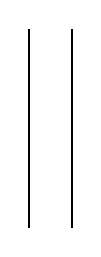
\begin{tikzpicture}[scale=.55,font=\scriptsize]
  \rooster{-2}{1}{3}{-1}{1}{3}
  \draw[thick] (0,-1.3) -- (0,3.3) (1,-1.3) -- (1,3.3);
\end{tikzpicture}}
\begin{center}\small Links snijden $x = 0$ en $y = 1$ elkaar op $l$; rechts zijn hun beelden evenwijdig.\end{center}

\begin{oefeningen}
\oef{h2-trans}
\end{oefeningen}

\subsection{De stelling van Pappus}

Pappus van Alexandrië bewees rond het jaar 320 een stelling die pas eeuwen later haar echte plaats kreeg: ze gaat alleen over punten op rechten, en is daarmee een van de eerste stellingen van de projectieve meetkunde. We bewijzen eerst een versie met evenwijdige rechten, en sturen daarna een rechte naar oneindig.

\figuren{\begin{tikzpicture}[scale=1.35,font=\scriptsize]
  \draw[thick] (-.2,0) -- (4,0) node[right] {$l$};
  \draw[thick] (-.2,1.85) -- (4,2.9) node[right] {$m$};
  \draw[grijs] (.8,0) -- (1.9,2.375) (.4,2) -- (2,0);
  \draw[grijs] (.8,0) -- (3.6,2.8) (.4,2) -- (3.4,0);
  \draw[grijs] (2,0) -- (3.6,2.8) (1.9,2.375) -- (3.4,0);
  \draw[accent,thick] (.9,.9) -- (3.1,1.2);
  \punt[below]{.8}{0}{A}
  \punt[below]{2}{0}{B}
  \punt[below]{3.4}{0}{C}
  \punt[above]{.4}{2}{A'}
  \punt[above]{1.9}{2.375}{B'}
  \punt[above]{3.6}{2.8}{C'}
  \fpunt[left]{1.24}{.95}{X}
  \fpunt[below]{1.84}{1.04}{Y}
  \fpunt[below right]{2.665}{1.164}{Z}
\end{tikzpicture}}
\begin{center}\small Pappus: $X = AB' \cap A'B$, $Y = AC' \cap A'C$ en $Z = BC' \cap B'C$ liggen op één rechte.\end{center}

\begin{theorie}
\begin{stelling}{Pappus, evenwijdige vorm}
Liggen $A$, $B$ en $C$ op een rechte $l$ en $A'$, $B'$ en $C'$ op een rechte $m$, allemaal verschillend van het snijpunt van $l$ en $m$, en is $AB' \parallel A'B$ en $AC' \parallel A'C$, dan is ook $BC' \parallel B'C$.
\end{stelling}

\begin{bewijs}
\textit{$l$ en $m$ snijden elkaar in $O$.} Neem een affien assenstelsel met oorsprong $O$, de $x$-as $l$ en de $y$-as $m$. Dan is $A(a, 0)$, $B(b, 0)$, $C(c, 0)$, $A'(0, a')$, $B'(0, b')$, $C'(0, c')$, met coördinaten die niet 0 zijn. Twee vectoren $(u_1, u_2)$ en $(v_1, v_2)$ zijn evenwijdig als $u_1v_2 - u_2v_1 = 0$, dus
\bewijsregel{AB' \parallel A'B \iff (-a, b') \parallel (b, -a') \iff aa' = bb' .}
Net zo is $AC' \parallel A'C \iff aa' = cc'$. Dan is $bb' = cc'$, en dat is $BC' \parallel B'C$.

\textit{$l \parallel m$.} Neem $l$ als $x$-as en een $y$-as met $m: y = 1$. Dan is $A(a, 0)$, \dots, $A'(a', 1)$, \dots, en
\bewijsregel{AB' \parallel A'B \iff (b' - a, 1) \parallel (b - a', -1) \iff a + a' = b + b' .}
Net zo geeft $AC' \parallel A'C$ dat $a + a' = c + c'$, dus $b + b' = c + c'$: $BC' \parallel B'C$.
\end{bewijs}
\end{theorie}

\begin{theorie}
\begin{stelling}{Pappus}
Liggen $A$, $B$ en $C$ op een rechte $l$ en $A'$, $B'$ en $C'$ op een rechte $m$, allemaal verschillend van het snijpunt van $l$ en $m$, dan liggen

\vspace{1mm}
\qquad $X = AB' \cap A'B$, \quad $Y = AC' \cap A'C$, \quad $Z = BC' \cap B'C$

\vspace{1mm}
op één rechte.
\end{stelling}

\begin{bewijs}
$X$ ligt niet op $l$: anders lag het snijpunt van $AB'$ met $l$, en dat is $A$, ook op $A'B$, en dan was $A = B$. Net zo liggen $X$ en $Y$ niet op $l$ of $m$, dus is de rechte $XY$ niet $l$ of $m$. Stuur $XY$ met een projectieve transformatie naar oneindig. Rechten blijven rechten, dus de beelden voldoen aan de voorwaarden van de evenwijdige vorm: $AB'$ en $A'B$ snijden elkaar op oneindig, en ook $AC'$ en $A'C$. Dus zijn ook de beelden van $BC'$ en $B'C$ evenwijdig: ze snijden elkaar op de rechte op oneindig. Terug naar het origineel: $Z$ ligt op $XY$.
\end{bewijs}
\end{theorie}

Het idee van dit bewijs komt vaak terug: kies de rechte die je wilt bewijzen als rechte op oneindig, en het probleem wordt een eigenschap over evenwijdige rechten.

\voorbeeld{}{Neem $A(1, 0)$, $B(2, 0)$, $C(3, 0)$ op de $x$-as en $A'(0, 3)$, $B'(0, 2)$, $C'(0, 1)$ op de $y$-as. Bereken $X$, $Y$ en $Z$, en controleer Pappus.\label{vb:h2-pappus}}{%
\uitleg{Bereken de zes rechten met het vectorproduct, en daarna de drie snijpunten.}
\begin{stappenbreed}
AB' = \rc{-2}{-1}{2}, \quad A'B = \rc{3}{2}{-6} & De eerste twee rechten. \\[1ex]
X = (2, -6, -1) \sim \hc{-2}{6}{1} & $X(-2, 6)$. \\[1ex]
AC' = \rc{-1}{-1}{1}, \quad A'C = \rc{3}{3}{-9} & $x + y = 1$ en $x + y = 3$. \\[1ex]
Y = (6, -6, 0) \sim \hc{1}{-1}{0} & $AC' \parallel A'C$: $Y$ ligt op oneindig. \\[1ex]
BC' = \rc{-1}{-2}{2}, \quad B'C = \rc{2}{3}{-6} & De laatste twee. \\[1ex]
Z = \hc{6}{-2}{1} & $Z(6, -2)$. \\[1ex]
\begin{vmatrix} -2 & 6 & 1 \\ 1 & -1 & 0 \\ 6 & -2 & 1 \end{vmatrix} = -2 \cdot (-1) - 6 \cdot 1 + 1 \cdot 4 = 0 & Op één rechte.
\end{stappenbreed}
De rechte $XZ$ is $x + y = 4$, met richting $(1, -1)$: ze gaat inderdaad door het punt op oneindig $Y$.}

\begin{oefeningen}
\oef{h2-pappus}
\end{oefeningen}

\subsection{Terug naar het probleem}

\voorbeeld{}{Terug naar het probleem. Een schilder zet een vloer met vierkante tegels op zijn doek. De voegen die van hem weg lopen, zijn op de vloer evenwijdig, maar op het doek lopen ze samen in één punt $V$. Ook de diagonalen van de tegels lopen samen, in een ander punt $D$. Het oog staat op hoogte 1 boven de vloer en het doek op afstand 1. Schrijf het perspectief van de vloer op het doek als een projectieve transformatie. Waar komt de rechte op oneindig van de vloer terecht? Waar liggen $V$ en $D$, en waarom liggen ze op één horizontale rechte, de horizon? Bestaat er een meetkunde waarin evenwijdige rechten elkaar echt snijden?\label{vb:h2-terug}}{%
\uitleg{Een punt van de vloer heeft coördinaten $(X, Z)$: opzij en diep. Het ligt in de ruimte in $(X, -1, Z)$, en komt op het doek in $\bigl(\tfrac XZ, -\tfrac1Z\bigr)$.}
\begin{stappenbreed}
(X, Z) \mapsto \Bigl(\frac XZ, -\frac1Z\Bigr) = \hc{X}{-1}{Z} & Homogeen op het doek. \\[2ex]
\kol{x \\ y \\ w} = \um{rrr}{1 & 0 & 0 \\ 0 & 0 & -1 \\ 0 & 1 & 0}\kol{X \\ Z \\ W} & Met $W = 1$ voor gewone vloerpunten; $\det A = 1$. \\[4ex]
\hc XZ0 \mapsto \hc X0Z & De rechte op oneindig van de vloer gaat naar $y = 0$: de horizon. \\[1ex]
\hc010 \mapsto \hc001 = V(0, 0) & De voegen in de diepte, richting $(0, 1)$. \\[1ex]
\hc110 \mapsto \hc101 = D(1, 0) & De diagonalen, richting $(1, 1)$. \\[1ex]
\hc100 \mapsto \hc100 & De dwarse voegen blijven evenwijdig.
\end{stappenbreed}}

Dat beantwoordt alle vragen. De punten op oneindig van de vloer vormen een rechte, en het perspectief is een projectieve transformatie: die stuurt rechten naar rechten. Dus liggen de beelden van alle punten op oneindig van de vloer op één rechte van het doek, de horizon. Het verdwijnpunt $V$ ligt recht voor het oog, en het verdwijnpunt $D$ van de diagonalen ligt even ver opzij als het doek van het oog staat. Schilders noemden $D$ het \emph{afstandspunt}: Leon Battista Alberti beschreef in 1435 hoe je er een tegelvloer mee tekent. En de meetkunde waarin evenwijdige rechten elkaar echt snijden, bestaat: het is het projectieve vlak. Wat op de vloer oneindig ver ligt, ligt op het doek op de horizon, en omgekeerd gaat de rechte van de vloer recht onder het oog ($Z = 0$) naar de rechte op oneindig van het doek. Voor een projectieve transformatie is \textit{oneindig ver} geen bijzondere plaats.

\begin{oefeningen}
\oef{h2-terug}
\end{oefeningen}

%========================================================================================
\opdrachtenkop

\begin{oefeningen}
\oef{h2-o1}

\oef{h2-o2}

\oef{h2-o3}

\oef{h2-o4}

\oef{h2-o5}

\oef{h2-o6}

\oef{h2-o7}

\oef{h2-o8}

\oef{h2-o9}

\oef{h2-o10}

\oef{h2-o11}

\oef{h2-o12}

\oef{h2-o13}

\oef{h2-o14}

\oef{h2-o15}

\oef{h2-o16}

\oef{h2-o17}

\oef{h2-o18}

\oef{h2-o19}

\oef{h2-o20}

\oef{h2-o21}
\end{oefeningen}

%----------------------------------------------------------------------------------------
% KOPPEL: verbanden met andere leerstof
%----------------------------------------------------------------------------------------
\needspace{20\baselineskip}
\opdrachtsectie{Koppel}

\lkr{Ruimtemeetkunde staat in het 6de jaar van pakket 4. Getaltheorie (rekenen modulo $n$) en Groepen zijn modules van het 6de jaar: kijk na of ze al gezien zijn.}

\begin{oefeningen}
\oef{h2-koppel-1}

\oef{h2-koppel-2}

\oef{h2-koppel-3}
\end{oefeningen}

%----------------------------------------------------------------------------------------
\needspace{40\baselineskip} % de test en het schema Fout? Herhaal samen op een pagina
\opdrachtsectie{Test jezelf}

\begin{oefeningen}
\oef{h2-t1}

\oef{h2-t2}

\oef{h2-t3}

\oef{h2-t4}

\oef{h2-t5}

\oef{h2-t6}

\oef{h2-t7}
\end{oefeningen}

\herhaalschema{%
  \fv{oef:h2-t1}{vb:h2-hc}{oef:h2-hc}%
  \fv{oef:h2-t2}{vb:h2-rechte}{oef:h2-rechte}%
  \fv{oef:h2-t3}{vb:h2-snij}{oef:h2-snij}%
  \fv{oef:h2-t4}{vb:h2-verbind}{oef:h2-snij}%
  \fv{oef:h2-t5}{vb:h2-det}{oef:h2-det}%
  \fv{oef:h2-t6}{vb:h2-verdwijn}{oef:h2-persp}%
  \fv{oef:h2-t7}{vb:h2-trans}{oef:h2-trans}}

\ifzelfstudie
\section*{Maak je eigen samenvatting}
Sluit dit boek en schrijf in je schrift: waar het verdwijnpunt van een richting ligt, wat het projectieve vlak is en waarom twee rechten er altijd één snijpunt hebben, homogene coördinaten van punten (ook op oneindig) en van rechten, het snijpunt en de verbindingsrechte met het vectorproduct, de tests met een determinant, het dualiteitsprincipe, de stellingen van Desargues en Pappus met het idee van hun bewijs, en wat een projectieve transformatie is. Vergelijk daarna met de kaders.
\fi
